%%% Thesis Style
%%% Jonas Schöley
%%% 2020-10-26

%--- Documentclass -----------------------------------------------------

\documentclass[10pt, twoside]{article}
\raggedbottom

%--- Font/encoding -----------------------------------------------------

\usepackage[utf8]{inputenc}       % .tex-file text encoding
\usepackage[T1]{fontenc}          % vector fonts and special chars in output

%--- Maths -------------------------------------------------------------

\usepackage{amsmath}  % various maths features
\usepackage{amssymb}  % maths symbols
\usepackage{mathrsfs} % maths script fonts
\usepackage{newtxtext, newtxmath} % Times Roman font family

%--- Links -------------------------------------------------------------

\usepackage{hyperref}
\hypersetup{
  hidelinks=true,
  breaklinks=true,
  colorlinks=false,
  pdftitle={The gestational age pattern of feto-infant mortality}
}
\urlstyle{rm}

%--- Misc --------------------------------------------------------------

\usepackage{etoolbox}  % allows to inject commands inside environments
%\usepackage{placeins} % control the placement of floats via \FloatBarrier
\usepackage{float}     % control placement of floats
\usepackage{xcolor}    % for colored links

%--- Figures -----------------------------------------------------------


  \usepackage{graphicx} % include external images
  \floatplacement{figure}{H}

  % generate all images so they have a width \cnstmaxfigwidth
  % images get their normal width if they fit onto the page
  % images are scaled down if they would overflow the margins
  \makeatletter
    \def\cnstmaxfigwidth{
      \ifdim \Gin@nat@width>\linewidth
        \linewidth
      \else \Gin@nat@width
      \fi
    }
  \makeatother
  \let\Oldincludegraphics\includegraphics
  \renewcommand{\includegraphics}[1]{\Oldincludegraphics[width=\cnstmaxfigwidth]{#1}}

  %\AfterEndEnvironment{figure}{\FloatBarrier}


%--- Captions ----------------------------------------------------------

\usepackage{caption}
\DeclareCaptionLabelSeparator{capsep}{:\hspace{0.2cm}}
\captionsetup[figure]{
            labelsep        = capsep,
            name            = Figure,
            font            = {rm, small},
            labelfont       = bf,
            justification   = justified,
            singlelinecheck = true,
            indention       = 0.5cm
}
\captionsetup[table]{
            labelsep        = capsep,
            name            = Table,
            font            = {rm, small},
            labelfont       = bf,
            justification   = justified,
            singlelinecheck = true,
            indention       = 0.5cm
}

% captions above
\floatstyle{plaintop}
\restylefloat{table}
\restylefloat{figure}

%--- Localization ------------------------------------------------------

% babel
\usepackage[english]{babel} % document language/localization
\usepackage[htt]{hyphenat}  % hyphenation rules

%--- Bibliography ------------------------------------------------------

\usepackage{natbib}
\setcitestyle{aysep={}}
\bibliographystyle{abbrvnat}
\newcommand{\doi}[1]{\href{http://www.dx.doi.org/#1}{doi:#1}}

%--- General layout ----------------------------------------------------

\usepackage{geometry}
\geometry{
  paperheight = 24cm,
  paperwidth  = 17cm,
  top         = 2.54cm,
  bottom      = 2.54cm,
  inner       = 2cm,
  outer       = 2.54cm,
  footskip    = 11mm,
  headheight  = 1cm,
  headsep     = 0.75cm,
  showframe   = false
}

% change spacing
\setlength{\parskip}{0.5ex}
\setlength{\parindent}{0cm}
\setlength{\bibsep}{.18cm}

% no page numbers
\pagenumbering{gobble}

% avoid orphans and widows
\widowpenalty = 10000
\clubpenalty  = 10000

% don't break footnotes
\interfootnotelinepenalty = 10000

% don't hyphenate across pages
\brokenpenalty10000\relax

% increase fraction of page that can be used by floats
% before a pure float-page is created
\renewcommand{\floatpagefraction}{.8}

%--- Lists -------------------------------------------------------------

% tight lists
\providecommand{\tightlist}{%
  \setlength{\itemsep}{0pt}\setlength{\parskip}{0pt}}

%--- Sections ----------------------------------------------------------

% depth of table of content

% spacing
\makeatletter
\renewcommand\section{\@startsection {section}{1}{\z@}%
                                   {-24pt}%
                                   {2.3ex \@plus.2ex}%
                                   {\normalfont\large\bfseries}}
\renewcommand\subsection{\@startsection{subsection}{2}{\z@}%
                                     {-24pt}%
                                     {1.5ex \@plus .2ex}%
                                     {\normalfont\normalsize\bfseries}}
\makeatother

% style
\usepackage{titlesec}
\titleformat{\section}[hang]{\raggedright\normalfont\bfseries\large}{\thesection.}{1ex}{}
\titleformat{\subsection}[hang]{\raggedright\normalfont\bfseries}{\thesubsection}{1ex}{}
\titleformat{\subsubsection}[hang]{\raggedright\normalfont\bfseries}{\thesubsubsection}{1ex}{}

%--- Footnotes ---------------------------------------------------------

\usepackage[bottom]{footmisc}

% make linebreaks start under footnote label
\setlength{\footnotemargin}{0.3em}

\let\oldfootnote\footnote
\renewcommand\footnote[1]{%
\oldfootnote{\hspace{0.6mm}#1}}

%--- Tables ------------------------------------------------------------

  \usepackage{array,longtable,booktabs,multirow}
  % -- This is needed because raggedright in table elements redefines \\:
  \newcommand{\PreserveBackslash}[1]{\let\temp=\\#1\let\\=\temp}
  \let\PBS=\PreserveBackslash
  \usepackage{etoolbox} % global table format
  \AtBeginEnvironment{tabular}{\scriptsize}

%--- Code listings -----------------------------------------------------

  \usepackage{color}
  \usepackage{fancyvrb}
  \newcommand{\VerbBar}{|}
  \newcommand{\VERB}{\Verb[commandchars=\\\{\}]}
  \DefineVerbatimEnvironment{Highlighting}{Verbatim}{commandchars=\\\{\}}
  % Add ',fontsize=\small' for more characters per line
  \newenvironment{Shaded}{}{}
  \newcommand{\AlertTok}[1]{\textbf{#1}}
  \newcommand{\AnnotationTok}[1]{\textit{#1}}
  \newcommand{\AttributeTok}[1]{#1}
  \newcommand{\BaseNTok}[1]{#1}
  \newcommand{\BuiltInTok}[1]{#1}
  \newcommand{\CharTok}[1]{#1}
  \newcommand{\CommentTok}[1]{\textit{#1}}
  \newcommand{\CommentVarTok}[1]{\textit{#1}}
  \newcommand{\ConstantTok}[1]{#1}
  \newcommand{\ControlFlowTok}[1]{\textbf{#1}}
  \newcommand{\DataTypeTok}[1]{\underline{#1}}
  \newcommand{\DecValTok}[1]{#1}
  \newcommand{\DocumentationTok}[1]{\textit{#1}}
  \newcommand{\ErrorTok}[1]{\textbf{#1}}
  \newcommand{\ExtensionTok}[1]{#1}
  \newcommand{\FloatTok}[1]{#1}
  \newcommand{\FunctionTok}[1]{#1}
  \newcommand{\ImportTok}[1]{#1}
  \newcommand{\InformationTok}[1]{\textit{#1}}
  \newcommand{\KeywordTok}[1]{\textbf{#1}}
  \newcommand{\NormalTok}[1]{#1}
  \newcommand{\OperatorTok}[1]{#1}
  \newcommand{\OtherTok}[1]{#1}
  \newcommand{\PreprocessorTok}[1]{\textbf{#1}}
  \newcommand{\RegionMarkerTok}[1]{#1}
  \newcommand{\SpecialCharTok}[1]{#1}
  \newcommand{\SpecialStringTok}[1]{#1}
  \newcommand{\StringTok}[1]{#1}
  \newcommand{\VariableTok}[1]{#1}
  \newcommand{\VerbatimStringTok}[1]{#1}
  \newcommand{\WarningTok}[1]{\textit{#1}}
  \DefineVerbatimEnvironment{Highlighting}{Verbatim}{
    numbers=left,fontsize=\footnotesize,commandchars=\\\{\}
  }

%--- Subscripts --------------------------------------------------------


%--- Includes ----------------------------------------------------------

% header_includes
  \usepackage[section]{placeins}

%--- Title, authors ----------------------------------------------------

  \title{\large\textbf{The gestational age pattern of feto-infant mortality}\vskip 0em}
  \author{\normalsize\textrm{\textbf{Jonas Schöley\footnote{Interdisciplinary Centre on Population Dynamics, University of Southern Denmark. Correspondence: \href{mailto:jschoeley@health.sdu.dk}{\nolinkurl{jschoeley@health.sdu.dk}}. During the writing of this article the author was a guest at the Max-Planck Institute for Demographic Research and funded by a grant from AXA Insurance.}}}}
\date{\vspace{-5ex}}

%--- Print main text ---------------------------------------------------

\begin{document}

  \maketitle

\vspace*{-24pt}
\vspace*{5mm}



\hypertarget{introduction}{%
\section{Introduction}\label{introduction}}

The different segments of a birth cohort's mortality trajectory have been thoroughly mapped starting with the sudden decline in the risk of death after a peak at birth \citep[e.g.,][]{Bourgeois-Pichat1951, Galley1999, Berrut2016}, the arrival at minimum risk in late childhood \citep{Ebeling2018}, the ``hump-shaped'' excess mortality in adolescence \citep[e.g.,][]{Thiele1871, Goldstein2011, Remund2018} and the exponential increase in the mortality hazard over much of the adult life \citep[e.g.,][]{Gompertz1825} which eventually flattens \citep[e.g.,][]{Perks1932, Vaupel1997, Horiuchi1998} and then plateaus among the oldest-old \citep[e.g.,][]{Gampe2010, Barbi2018}. Similar investigations have been made concerning the changing mortality risk of the unborn child over the age of a pregnancy \citep[e.g.,][]{Shapiro1962, Bakketeig1978, Goldhaber1991, Carlson1999, Woods2009}.

Both survival scenarios, fetal and infant, meet at the point of birth but are nonetheless fundamentally separated by the use of different timescales. While prenatal mortality is indexed by gestational age, commonly measured as the weeks since the last menstrual period of the pregnant woman, the survival of those born alive is followed over chronological age, i.e., time since birth. Such a strict separation of populations along the dividing line of birth makes this critical transition invisible in the study of mortality, delegating to it either the role of a right censoring or a point of entry into the risk set. An alternative perspective allows bridging the feto-infant gap by situating birth within the lifecycle of a cohort of unborn children whose survival is tracked over the age of gestation into infancy. By marking the vital events of fetal death, birth and infant death on a common age scale the risky transition of birth becomes an event \emph{within} the temporal observation horizon and its effect on the survival of a cohort on the onset of life can be studied by defining a feto-infant mortality trajectory: the combined risk of fetal or infant death among all members of a conception cohort still alive at a given week of gestation.

\begin{figure}
\centering
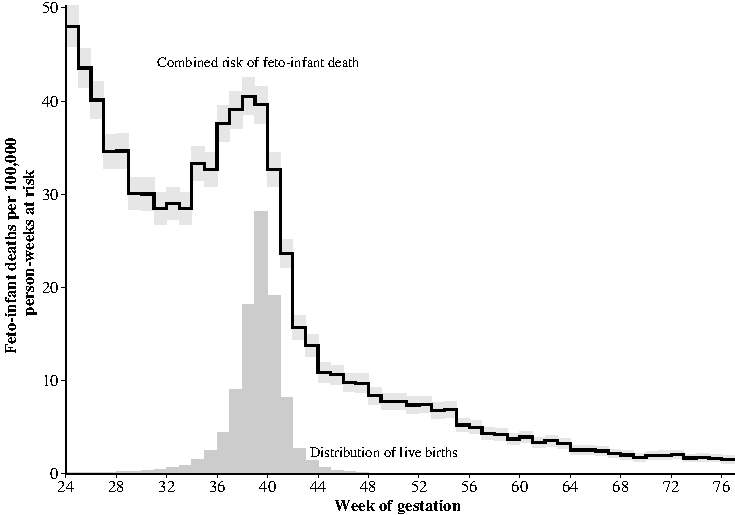
\includegraphics{fig/gestational_age_pattern.pdf}
\caption{\label{fig:gestational-age-pattern}The feto-infant mortality trajectory over gestational age for a U.S. cohort of fetuses conceived in 2009, surviving until fetal viability and followed over the next 52 weeks. The risk of feto-infant death among the survivors of the cohort declines exponentially over age interrupted only by a ``birth hump.''}
\end{figure}

Figure \ref{fig:gestational-age-pattern} shows gestation specific mortality rates for a cohort of children conceived in 2009 and either born or registered as an infant or fetal death in the U.S. The denominator of the rate is based upon all members of the conception cohort alive (either as fetus or infant) during a given week of gestation whereas the numerator includes all fetal- and infant deaths within the same week. The feto-infant mortality trajectory constructed from these rates thus measures the changing risk of \emph{any} adverse pregnancy outcome for the 52 weeks following gestational age 24, commonly defined as the ``limit of viability'' \citep{Seri2008}. The trajectory may be interpreted as the changing hazard of death for a cohort as its members pass the tumultuous transition period from fetus to infant. An exponential decline in mortality characterizes this period, interrupted only by hump-shaped excess mortality associated with the age-distribution of deliveries.

In this paper, descriptive findings on the feto-infant mortality trajectory and the associated phenomenon of a ``birth hump'' are presented.

Mortality trajectories that stretch across the feto-infant gap have been proposed several times but never entirely realized. In his seminal work on ``ontogenescence,'' -- the declining risk of death over age before maturity -- \citet{Levitis2011} considers the hazard of death on an age continuum from conception until adolescence with the event of birth acting as a ``transitional shock.'' By using a negative time scale before birth and positive after, Levitis implicitly assumes all births to occur at the same time post-conception -- a simplifying assumption which naturally leads to a spurious ``birth spike'' rather than a ``birth hump.'' \citet{Williamson2003} and \citet{Woods2009} model the cumulative risk of death of a cohort from conception until the first birthday and use weeks of gestation as time scale throughout the complete follow-up. As Williamson and Wood's model is based on previously published disjoint fetal- and infant lifetables, they too assume all births to take place at full-term.

The joint consideration of fetal and infant death is perhaps most prominently expressed in the perinatal mortality rate, commonly defined as the sum of all fetal deaths and infant deaths during the first seven days of life over the number of births within a year \citep{WHO2006}. The necessity for such a measure arose from the uncertainty regarding the classification of a death as stillborn or infant due to both varying legal requirements and the subjective judgment of the pediatrician. Designed as a simple and therefore widely applicable indicator, the perinatal mortality rate does not consider the time dimension of pregnancy, nor does it permit a survival analytic interpretation as the denominator is not the population at risk.

Fetal lifetables add both a time dimension and a survival interpretation to the analysis of pregnancy outcomes via the introduction of an ``ongoing pregnancies'' denominator \citep[e.g.,][]{Shapiro1962, French1962, Bakketeig1978, Goldhaber1991}. These life-tables report the probability of fetal death among the intrauterine survivors to some week of gestation. In an influential article \citet{Yudkin1987} advertise the use of a ``fetuses at risk'' denominator for the analysis of perinatal mortality by gestational age leading to a range of age-specific mortality indices that include compound fetal- and infant death endpoints \citep{Kristensen1992, Smith2001, Platt2004, Joseph2004, Smith2005, Joseph2007}. \citet{Kristensen1992} follows a cohort of fetuses from week 31 of gestation into infancy until week 76 and calculates a corresponding survival curve. The ratio of fetal- and neonatal\footnote{In this paper I use the term ``neonatal'' as referring to the first week of life.} deaths over fetuses at risk by week of gestation is advertised by \citet{Joseph2007} as the proper ``causal'' framework to the study of perinatal mortality. Making a similar argument \citet{Platt2004} propose a Cox regression model over age of gestation featuring a combined feto-infant death endpoint.

This paper contributes to the aforementioned literature on survival analysis \emph{around} the onset of life by studying the age pattern of mortality in a cohort of fetuses as they transition into infancy. A distinct phenomenon of this perinatal mortality trajectory is the ``birth hump.'' Via simple decomposition analysis, I show how fetal-, neonatal, and post-neonatal mortality and the probability of live birth all act together to form the ``hump.'' In a second step, I quantify the magnitude of the ``hump'' by proposing that the distinctive shape of feto-infant mortality on a cohort level is the result of two competing hazards: An ``ontogenescent'' hazard, due to causes with a declining incidence, and a ``transitional'' component, due to birth-related causes. I propose the probability of a fetus at 24 weeks of age to survive the following 12 months as a summary of the feto-infant mortality trajectory and ask how differences in this indicator across cohorts and between population strata are driven by changes in the shape of the gestational age pattern of feto-infant mortality.

\hypertarget{data-and-methods}{%
\section{Data and Methods}\label{data-and-methods}}

In this paper, I analyze U.S. fetal deaths, births, and infant deaths over the age of gestation. The data basis for this analysis consists of the birth certificates for the U.S. birth cohorts 1989/1990, 1999/2000, 2009/2010, the linked infant death certificates where applicable, and the fetal death certificates for the years 1989/1990, 1999/2000, and 2009/2010. Digitized versions of the certificates are provided by the National Center for Health Statistics in the form of the ``Birth Cohort Linked Birth -- Infant Death Data Files'' \citep{NCHS2016} and the ``Fetal Death Data Files'' \citep[see also \citet{Martin2002} for an introduction]{NCHS2016b}.

To analyze the gestational age mortality trajectory of a cohort of fetuses as they transition into life, I construct three conception cohorts of all fetuses conceived during the years 1989, 1999, and 2009 respectively. The 2009 cohort is further stratified by sex and maternal origin, two characteristics which are available on most birth-, fetal- and infant death certificates and serve to show how the phenomenon of the birth hump and the ontogenescent feto-infant mortality decline compares across key demographics.

Only fetuses who survived until week 24 of gestation, commonly defined as the ``age of viability,'' are considered in this study. Reporting guidelines and practice for fetal death vary across states. A left-truncation age of 24 serves to rectify these differences. It is chosen because based on evidence that under-reporting drastically increases already at week 23 \citep{Greb1987}\footnote{While their study dates back to 1987 I found evidence for the continued under-registration of fetal deaths in the U.S. prior to week 24 in the form of declining fetal death rates going from week 23 to 20 which lacks a biological explanation.}. Furthermore, a relatively late left-truncation age serves to minimize the bias due to the unknown numbers of induced abortions.

The initial size of the fetal-cohort at the beginning of week 24 is calculated via the ``extinct cohort'' method \citep{Bakketeig1978, Feldman1992} by adding all life-births within a conception cohort to all fetal deaths at weeks 24+. This is due to the simple observation that a life-birth at week of gestation \(t\) was a fetus prior to \(t\).

Using a multi-state lifetable, I follow the initial fetal population at week 24 for 52 weeks counting for each week \(t\) fetal deaths, neonatal deaths, post-neonatal deaths, and the corresponding population of survivors and their distribution across these three states. Distinguishing fetuses, newborns and infants who survived the first week of life then allows to decompose week-to-week changes in the combined feto-infant mortality rates \(m_t = \frac {\text{\# fetal or infant deaths at week}~t} {\text{Total feto-infant time at risk during week}~t}\) into changes due to a shifting distribution of fetuses, vs.~neonates vs.~post-neonates, and changes due to declining or increasing mortality rates within each state. Such a decomposition explains the ``birth hump'' in terms of the perinatal population dynamics. The Kitagawa method \citep{Kitagawa1955} is used to perform the decomposition.

\clearpage

\begin{table}
\begin{tabular}{p{5.9cm}p{5.9cm}} 
\toprule
\textbf{Ontogenescent component}
&
\textbf{Transitional component}
\\ 
\midrule
\textit{Ontogenescent hazard}
The instantaneous risk of fetal or infant death at gestational age $t=x+24$ due to causes with a continuously declining incidence.
$$
h^\mathrm{O}(x)=a_1\exp(-bx)
$$
&
\textit{Transitional hazard}
The instantaneous risk of fetal or infant death at gestational age x due to causes associated with the timing of onset of labor.
$$
h^\mathrm{T}(x)=a_2\exp\left(-\frac {(x-c)^2} {2\sigma^2}\right)
$$
\\
\textit{Cumulative ontogenescent hazard}
$$
H^\mathrm{O}(x) = \int_0^{x} h^\mathrm{O}(s)\,\mathrm{d}s = \frac {a_1 - a_1 \exp(-bx)} {b}
$$
&
\textit{Cumulative transitional hazard}
$$
H^\mathrm{T}(x) = \int_0^{x} h^\mathrm{T}(x)\,\mathrm{d}s = a_2 \sigma\sqrt{\pi/2}\left[\mathrm{erf}(A)+\mathrm{erf}(B)\right],
$$
where $A = \frac {c} {\sqrt{2}\sigma}$, $B = \frac {x-c} {\sqrt{2}\sigma}$, and $\mathrm{erf}(\cdot)$ is the Gaussian error function.

\\

$a_1$ \textit{Level of feto-infant mortality} The approximate hazard of feto-infant death at age of fetal viability.

&

$a_2$ \textit{Magnitude of birth hump} The instantaneous risk of fetal or infant death contributed by the birth-hump component at its peak.

\\

$b$ \textit{Rate of ontogenescence} The relative rate of feto-infant mortality decline over gestational age in absence of birth hump.

&

$c$ \textit{Location of birth hump}

The gestational age $t=c+24$ coinciding with the peak of the risk of fetal or infant death contributed by the birth-hump component.

\\

&

$\sigma$ \textit{Spread of transitional shock} The curvature of the risk of feto-infant death around its peak. Higher values flatten the birth hump.

\\ \midrule

\multicolumn{2}{c}{\textbf{Combined hazard}} \\ \midrule

\textit{Hazard of feto-infant death}
The instantaneous risk of fetal or infant death $x$ weeks past fetal viability.

&

$$
h(x) = h^\mathrm{O}(x) + h^\mathrm{T}(x)
$$

\\

\textit{Feto-infant survival curve} The probability of surviving $x$ weeks past fetal-viability.

&

$$
S(x) = \exp\left(-H^\mathrm{O}(x)-H^\mathrm{T}(x)\right)
$$

\\

\textit{Cumulative incidence of feto-infant death} Probability of fetal or infant death $x$ weeks past fetal-viability.

&

$$
F(x) = 1-S(x)
$$

\\ \midrule

\multicolumn{2}{c}{\textbf{Competing risks inference}} \\ \midrule

Cumulative incidence of feto-infant death due to causes associated with the timing of onset of labor.

&

$$
F^\mathrm{T}(x) = \int_0^x S(s)h^\mathrm{T}(s)\,\mathrm{d}s
$$

\\

Share of feto-infant deaths over $x$ weeks following fetal viability contributed by the "birth hump".

&

$$
\rho(x) = \frac {F^\mathrm{T}(x)} {F(x)}
$$

\\ \bottomrule

\end{tabular}
\caption{\label{tab:hazard-model} Parametric specification of the feto-infant mortality trajectory over age of gestation and derived quantities.}
\end{table}

\clearpage

Assuming a competing risks model (Table \ref{tab:hazard-model}) where death is either the result from causes which exhibit gradually declining incidence over gestation (e.g., extreme prematurity, in-utero fatalities due to congenital anomalies) or from causes increasing in incidence as full-term approaches (e.g., obstetric causes), I quantify the share of fetal- or infant deaths over the one-year follow-up from fetal viability which can be attributed to the ``birth-hump.''

I define \(F(52)\), the probability for a fetus alive at the 24th week of pregnancy to die in the following year, as a summary indicator of adverse pregnancy outcomes. In order to elucidate how the ``shape'' of the feto-infant hazard trajectory determines population differences in overall feto-infant death counts, I decompose differences in \(F(52)\) between two populations into differences due to the initial magnitude of mortality at the age of fetal viability, differences due to the rate of mortality decline over gestational age, and differences due to the location, shape, and magnitude of the ``birth hump'' component. This decomposition is performed via the Horiuchi decomposition \citep{Horiuchi2008} of the differences in \(F(52)\) as predicted by the model outlined in Table \ref{tab:hazard-model}.

\hypertarget{results}{%
\section{Results}\label{results}}

\hypertarget{feto-infant-population-dynamics-over-gestational-age}{%
\subsection{Feto-infant population dynamics over gestational age}\label{feto-infant-population-dynamics-over-gestational-age}}

The gestational age trajectory of feto-infant mortality as shown in Figure \ref{fig:perinatal-popdynamics}A may be segmented into a decline from week 24 to 33, a steep increase from week 33 to 39, a steep decrease from week 39 to 45, and a more gradual decrease over weeks 45 to 72. Throughout these four segments, the population composition shifts from a cohort of fetuses to a cohort with a substantial share of neonates to a cohort entirely composed of postneonates. Fetal mortality rates decline until week 32 and start to increase drastically into post-term, neonatal mortality declines until week 40, and then plateaus and post-neonatal mortality declines continuously over the entire observation period (Figure \ref{fig:perinatal-popdynamics}B). As shown by the Kitagawa decomposition in Table \ref{tab:perinatal-popdynamics}, the particular shape of the feto-infant mortality trajectory is the result of both the aforementioned changes in composition and rates.

\emph{Weeks 25 to 33: pre-term decline.} Feto-infant mortality declines by 34.6 percent over the nine weeks following the age of fetal-viability. The overwhelming share of the decline can be attributed to the lessening burden of prematurity reflected in the 95.7\% decline of neonatal mortality: Infants born at week 25 have a risk of death elevated by a factor of 654 compared to the fetal population at the same age whereas at week 33 this neonate penalty is reduced to a factor of 35.8. However, the increasing share of neonates from less than a percent to 1.9 percent counterbalances the effect of the reduction in neonatal mortality on the differential in feto-infant mortality.

\emph{Weeks 33 to 39: increase towards full-term.} Approaching full-term, feto-infant mortality reverses its trend and increases by 38.9 percent. Part of this increase is due to the increase in fetal death rates by more than 144 percent, an effect that is, in turn, mediated by the declining share of the fetal population in the cohort by 51.7 percent. Neonatal mortality rates continue to be higher compared to fetal mortality prior to week 39 (Figure \ref{fig:perinatal-popdynamics}C), and thus the rapidly increasing share of newborns contributes to the increase in combined feto-infant mortality.

\emph{Weeks 39 to 45: post-term decline.} While mortality increases post-term for both fetuses and neonates, it is the quickly vanishing share of both sub-populations that, along with declining rates of post-neonatal mortality, drives the steep decline in feto-infant mortality following full-term.

\emph{Weeks 45 to 72: post-neonatal decline.} With no remaining fetuses or neonates in the population, the feto-infant mortality trajectory is completely determined by the declining mortality of the post-neonatal population.

\vspace{2cm}

\begin{table}[b!]
\begin{tabular}{p{1.1cm}*{9}{p{0.75cm}}p{0.75cm}p{0.75cm}p{0.75cm}p{0.75cm}p{0.75cm}p{0.75cm}p{0.75cm}p{0.75cm}p{0.75cm}p{0.75cm}p{0.75cm}p{0.75cm}p{0.75cm}p{0.75cm}p{0.75cm}p{0.75cm}p{0.75cm}p{0.75cm}} 
\toprule
\textbf{Week} & \textbf{25} & $\rightarrow$ &
                \textbf{33} & $\rightarrow$ &
                \textbf{39} & $\rightarrow$ &
                \textbf{45} & $\rightarrow$ &
                \textbf{72} \\
\midrule
\multicolumn{10}{l}{\textbf{Mortality by stratum} in deaths per 100,000 person-weeks exposure} \\
Fetus        & 25.6   & \emph{(-22.4)} &
               19.9   & \emph{(+144)}  & 
               48.6   & \emph{(+128)}  &
               111.1  & $\cdot$ &
               $\cdot$ \\
Neonatal     & 16,774 & \emph{(-95.7)} &
               713    & \emph{(-94.2)} & 
               41.2   & \emph{(+53.5)} & 
               63.2   & $\cdot$ &
               $\cdot$ \\
Postneonatal & 6,392  & \emph{(-97.1)} &
               187    & \emph{(-87.1)} &
               24.1   & \emph{(-59.3)} &
                9.8   & \emph{(-78.8)} &
                2.1 \\
\multicolumn{10}{l}{\textbf{Relative exposure by stratum}} \\
Fetus        & .998  & \emph{(-2.6)}   &
               .973  & \emph{(-51.7)}  &
               .470  & \emph{(-98.9)}  &
               .005  & \emph{(-100)}   &
                0 \\
Neonatal     & <.001  & \emph{(+732)}   &
                .008  & \emph{(+2901)}  &
                 23.2 & \emph{(-97.6)}  &
                .006  & \emph{(-100)}   &
                0 \\
Postneonatal & <.001 & \emph{(+5,130)} &
                .019 & \emph{(+1443)}  &
                .298 & \emph{(+232)}   &
                .989 & \emph{(+1.1)}   &
                1 \\
\midrule
\multicolumn{10}{l}{\textbf{Combined feto-infant mortality}} \\
 & 43.6 & \emph{(-34.6)} &
   28.5 & \emph{(+38.9)} &
   39.6 & \emph{(-73.2)} &
   10.6 & \emph{(-80.4)} &
   2.1 \\
\multicolumn{10}{l}{\textbf{Absolute change in feto-infant mortality} due to differences in} \\
Composition & & +121.2 & & +96.7 & & -37.2 & & -0.39 & \\
Rates & & -136.3 & & -85.6 & & +8.2 & & -8.2 & \\
\midrule
Total $\Delta$ & & -15.1 & & +11.1 & & -28.9 & & -8.6 & \\
\bottomrule

\end{tabular}
\caption{\label{tab:perinatal-popdynamics} Decomposition of the change in combined feto-infant mortality over gestational age into contributions due to changing risk of death among fetuses, newborns, and post-neonates and the changing structure of the population along these dimensions. Percent relative change is given in parenthesis.}
\end{table}

\begin{figure}
\centering
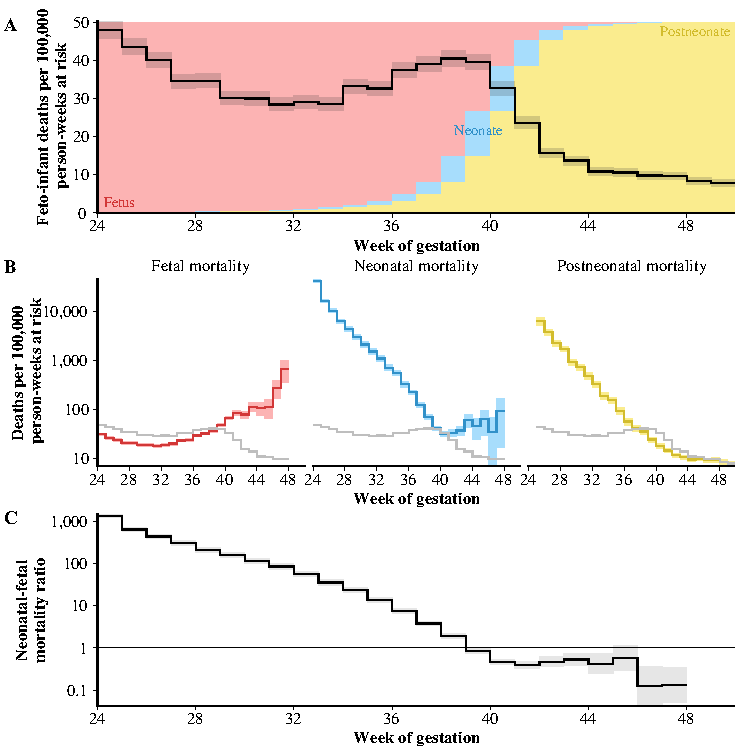
\includegraphics{fig/perinatal_popdynamics.pdf}
\caption{\label{fig:perinatal-popdynamics}Rates of fetal death, neonatal death, and post-neonatal death over weeks of gestational age as calculated for the cohort of U.S. fetuses conceived in 2009. The shaded background shows the distribution of survivors among the three states.}
\end{figure}

\clearpage

\hypertarget{stratum-specific-feto-infant-mortality-trajectories}{%
\subsection{Stratum-specific feto-infant mortality trajectories}\label{stratum-specific-feto-infant-mortality-trajectories}}

Males have a higher probability of death in the 52 weeks following fetal viability (Figure \ref{fig:perinatal-hazards}A). Out of 100,000 male fetuses of the 2009 U.S. conception cohort surviving until 24 weeks of gestation 851--878\footnote{I report the 95 percent prediction interval around the estimates.} (one out of 114--116) will not survive the following year, compared to 739--763, (one out of 131--135) female deaths over the same period. Thus, the male probability of feto-infant death is 12.6--17.8 percent higher than that of females. Most of this difference in survival is explained by a higher hazard level in males as measured by the \(a_1\) parameter: Ignoring the slightly earlier peak of the birth hump in males, the male hazard of feto-infant death is consistently higher across the 52 weeks of post-viability gestational age. The hazard of feto-infant death declines with a rate of 6.5--6.8 percent per additional week of gestation for males and 7.0--7.3 percent for females. The higher rate of ontogenescence among females substantially contributes to the sex-difference in one-year post-viability survival, while different magnitude and spread of the ``birth hump'' exhibit only a marginal and non-significant contribution. For additional parameter estimates see Tables \ref{tab:para-sex} and \ref{tab:hour-sex}.

Feto-infant survival improves considerably in the U.S. from 1989 to 2009. Out of 100,000 fetuses conceived in 1989 and reaching the age of viability 1,196--1,219 (one in 82--84), do not survive the following 52 weeks. This number drops to 969--990 (one in 101--103) deaths for the 1999 cohort and further down to 800--818 (one out of 122--125) deaths for conceptions in 2009. The 17.8--20.1 percent improvement in feto-infant survival between 1989 and 1999 is mainly explained by an increase in the rate of ontogenescence from approximately 6.1--6.2 percent per additional week of gestation to 7.0--7.2 percent and by a drop in the level of feto-infant mortality from 63--65 to 56--58 deaths per 100,000 person-weeks of exposure at fetal-viability. While the location of the peak ``birth-hump'' shifts into earlier gestation by about a week, neither magnitude nor spread of the hump change substantially between cohorts 1989 and 1999. Hence, the contribution of the transitional component to the overall improvement in one-year post-viability survival is small.

A different picture emerges for the 16.1--18.6 percent improvement in feto-infant survival between conception cohorts 1999 and 2009, which is primarily driven by a decline in the level of feto-infant mortality from 56--58 to 46--48 deaths per 100,000 person-weeks of exposure at fetal-viability. A substantial reduction in the magnitude of the birth hump from a peak value of 32--35 deaths per 100,000 person-weeks of exposure to 23--25 further contributes to the survival improvements while the rate of ontogenescence remains nearly constant.

\clearpage

\begin{figure}
\centering
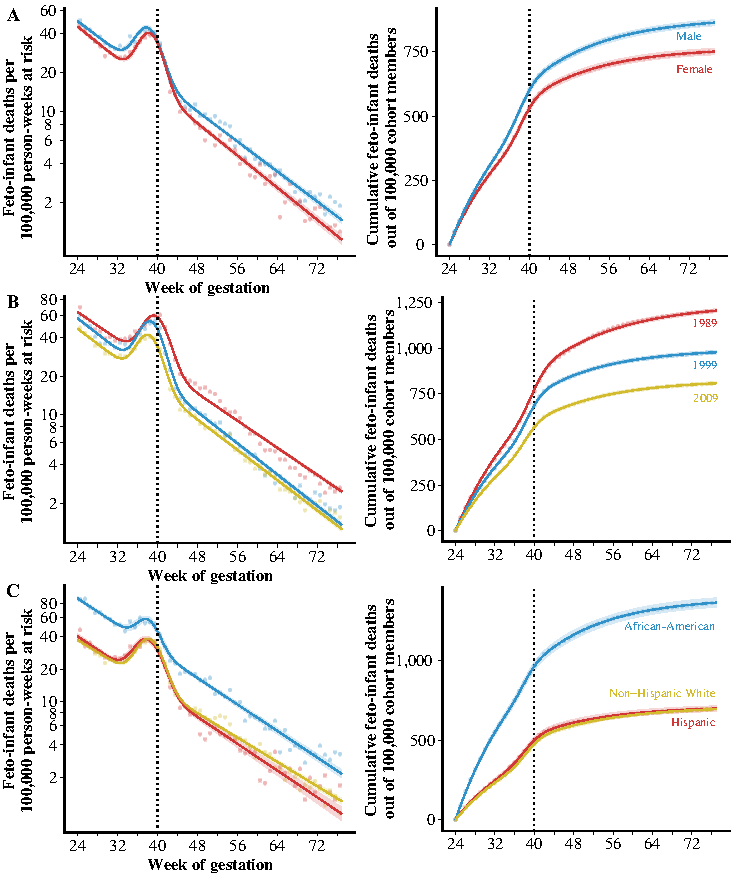
\includegraphics{fig/perinatal_hazards.pdf}
\caption{\label{fig:perinatal-hazards}Age trajectories of feto-infant survival A) by sex for the U.S. conception cohort 2009, B) by U.S. conception cohort, C) by maternal origin for the U.S. conception cohort 2009. Fitted (lines) versus lifetable estimates (points).}
\end{figure}

\clearpage

There are considerable differences in feto-infant survival by ethnicity of the mother with the hazard of feto-infant death for the cohort of African-American origin consistently being greater than the hazards for the cohort of Hispanic or Non-Hispanic White origin (Figure \ref{fig:perinatal-hazards}C). In the U.S. conception cohort 2009, out of 100,000 fetuses of African-American origin at pregnancy week 24 an estimated 1,332--1,399 (one in 71--75) either die in-utero or as infants in the following year compared to 679--719 (one in 139--147), and 684--705 (one in 142--146) for fetuses of Hispanic and non-Hispanic white origin respectively. Virtually all of the differences in feto-infant survival between the African-American stratum and the White/Hispanic origin strata are due to differences in the hazard level. Notably, the share of deaths attributable to the birth-hump is substantially lower in the African-American stratum (7.5--11.0 percent) compared to the Hispanic (18.7--24.4 percent) and non-Hispanic White (19.1--21.7 percent) strata. For further details see Tables \ref{tab:para-origin} and \ref{tab:hour-origin}.

\hypertarget{discussion}{%
\section{Discussion}\label{discussion}}

With the advent of modern obstetric practice, the distinction between fetus and infant stage became malleable and a question of optimal choice: Should we deliver early? Should we perform surgery in-utero? Should we try to prolong the pregnancy? Better and more widely employed prenatal diagnostics made the uterus almost transparent\footnote{In quite a real sense if one considers the images generated from a 3D ultrasound.}. The feto-infant distinction lost relevance as available knowledge about the degree of maturity, and the presence of congenital disorders informed the future survival prospects of the child, in-utero or not. \citet{Isaacson1996}, in a historical study of obstetric texts, identified the ``creation of the fetus-infant'' -- a being separate from the pregnant woman and endowed with a history that begins before birth. The consideration of the feto-infant mortality trajectory over age of gestation naturally arises from the continued blurring of lines that divide the stages of existence. But what does the feto-infant as a concept contribute to the study of mortality? 1. a more realistic quantification of undesired pregnancy outcomes, 2. the phenomenon of a ``birth hump,'' and on a related note, 3. the possibility to model the risk associated with the transition of birth.

\emph{Quantifying undesired pregnancy outcomes:} A sole focus on rates of infant mortality, fetal mortality or perinatal mortality hides the true incidence of adverse pregnancy outcomes, and the incompatible definition of these measures prohibits to form a simple sum which more truthfully reflects on the loss of life within a pregnancy cohort. By employing the methods of survival analysis, I have calculated that one out of 73 African-American women who conceived in 2009 and continued their pregnancy to the 24th week of gestation are expected to lose their child in the following year. Not only shows this number the continued racial disparity in the prospects of survival at the onset of life when compared to the population average of one in 124; would pregnancy come with the same warnings as prescription drugs, feto-infant death past the age of fetal viability would have to be labeled as a ``common'' side effect according to the standards put forth in \citet{CIOMSWGIIIV1999}.

\emph{The phenomenon of the ``birth hump'':} Former bio-demographic analyses and descriptions of the age trajectories of combined feto-infant mortality suffered either from a lack of data, the authors being forced to rely instead on rough assumptions and combinations of observations from various populations \citep{Williamson2003, Woods2009, Levitis2011, Berrut2016}. The detailed micro-data on fetal deaths, births, and infant deaths in the U.S. allowed me to calculate the mortality trajectory of various fetal cohorts as they transition into infancy. Interestingly, the asymmetric sigmoid-shape for the cumulative distribution of feto-infant deaths around term, proposed by \citet{Williamson2003} on the grounds of theoretical considerations, is supported by the data presented here and it can be derived from the assumption of an exponentially declining hazard component added to a hazard component with a Gaussian shape. Under a simple competing risks model, less than 20 percent of feto-infant deaths during the one-year follow-up from the age of fetal viability are contributed by the ``birth hump.'' Notably, among the conception cohort of African-American maternal origin, this contribution is only 9 percent, while the general level of feto-infant mortality is much higher among this stratum compared to the population average. This suggests that the ``hump'' is an additive phenomenon, which in turn implies an increasing share of deaths during or shortly after labor on all fetal and infant death as feto-infant mortality continues to decline.

\emph{Risks associated with the transition of birth:} A formidable challenge for future research is to connect the aggregate phenomenon of the ``birth-hump'' to the transitional shock experienced by an individual as it moves from the intrauterine environment into infancy. In perinatal epidemiology, the same estimation problem is motivated by the desire to maximize the survival chances of an unborn child. Should labor be induced at a given age of gestation, or is it better to wait until labor sets in naturally? At heart lies the question of the risk of death prior to and after delivery, but such a change in risk can only ever be estimated indirectly as no one born alive ever died in utero. Current approaches to calculating the ``risk of birth'' thus are based on the strong assumption that children born in a given week of gestation \(t\) experienced the same risk of fetal death as the complete cohort of unborn children until \(t\). But given that some fetal conditions are associated with a higher risk of stillbirth, pre-term birth, and infant death, this assumption must be deemed very crude, and instead, one would expect prematurely born infants to have had a higher risk of fetal death compared to infants born on full-term. Including exactly those information on fetal condition into the model, which are strongly associated with the timing of birth as well as fetal and infant death, would alleviate this issue and allow for a more precise estimate of the change in mortality across the feto-infant transition conditional on the timing of birth. The methodological framework for such an analysis could be given by the multi-timescale and multi-state approach to survival analysis, as proposed by \citet{Iacobelli2013}.

\clearpage

\hypertarget{appendix-appendix}{%
\appendix}


\hypertarget{description-of-methods}{%
\section{Description of methods}\label{description-of-methods}}

\hypertarget{determining-gestational-age}{%
\subsection*{Determining gestational age}\label{determining-gestational-age}}
\addcontentsline{toc}{subsection}{Determining gestational age}

For the purposes of this paper, a key field on the birth and death certificates is the estimated age of gestation upon delivery as a proxy for the length of a pregnancy. This measure is subject to certain biases, which are crucial to keeping in mind when interpreting the results.
Gestational age is defined as the weeks since the first day of the last menstrual period of the mother (LMP) and commonly measured by subtracting the date at LMP as reported by the women from the date of (still-)birth. This method suffers from recall bias, which may lead to digit preference in the reported dates. An alternative ist to derive the age of a pregnancy from ultrasound measurements of the unborn child. While the ultrasound method generally allows for a more precise estimate of the date of life-birth, it can be systematically biased in cases where the fetus is growth restricted. As abnormal fetal growth is a risk factor for fetal death, the gestational age at stillbirth may be severely biased under the ultrasound method. Additionally, the age of gestation at fetal death is positively biased by the time-lag between intrauterine death and the delivery of the dead fetus, which in-part explains the observation of fetal deaths at the implausible gestational ages of 46 and 47 weeks.
In analyzing the age pattern of feto-infant mortality, I will utilize the gestational ages at delivery as they are reported on the birth and fetal death certificates and point out the role of the aforementioned biases whenever they are relevant for the interpretation of the results.

\hypertarget{delineating-conception-cohorts}{%
\subsection*{Delineating conception cohorts}\label{delineating-conception-cohorts}}
\addcontentsline{toc}{subsection}{Delineating conception cohorts}

When considering the survival of fetuses into infancy, a straightforward definition of a cohort is all subjects who have been conceived during the same time period, i.e., a ``conception cohort.'' To determine the year of conception \(y\) for every single subject in the data I subtract the estimated weeks of gestation at delivery from the date at delivery and add two weeks to account for the average delay between the date of the last menstrual period of the mother (the time origin of the gestational age) and the date of fertilization. In this paper, I compare conception cohorts 1989, 1999, 2009.

\hypertarget{assembling-the-multi-state-feto-infant-life-table}{%
\subsection*{Assembling the multi-state feto-infant life table}\label{assembling-the-multi-state-feto-infant-life-table}}
\addcontentsline{toc}{subsection}{Assembling the multi-state feto-infant life table}

After delineating the conception cohorts \(y\) and determining \(N^{F}_{24}\), the number of fetuses at risk at the start of observation, I calculate a multi-state feto-infant life table across the five states of fetus \(F\), neonate \(N\), post-neonate \(P\), dead \(D\) and censored \(C\). This requires the aggregation of transition counts \(T\) among states over age. For each single week of gestation let \(T_{t}^{F\rightarrow D}\) denote the number of fetal deaths, \(T_{t}^{F\rightarrow N}\) the number of births, \(T_{t}^{N\rightarrow D}\) the number of neonatal deaths, \(T_{t}^{N\rightarrow P}\) the number of recent survivors of the first week of life, \(T_{t}^{P\rightarrow D}\) the number of post-neonatal deaths, and \(T_{t}^{P\rightarrow C}\) the number of censorings at week 77. The fetal, neonatal and post-neonatal population at risk at the beginning of gestational age \(t\) are then given by the recurrence equations

\[
\begin{aligned}
N_{t}^{F} &= N_{t-1}^{F} - T_{t-1}^{F\rightarrow D} - T_{t-1}^{F\rightarrow N}, \\
N_{t}^{N} &= N_{t-1}^{N} + T_{t-1}^{F\rightarrow N} - T_{t-1}^{N\rightarrow D} - T_{t-1}^{N\rightarrow P}, \\
N_{t}^{P} &= N_{t-1}^{P} + T_{t-1}^{N\rightarrow P} - T_{t-1}^{P\rightarrow D} - T_{t-1}^{P\rightarrow C}.
\end{aligned}
\]

To calculate the population exposures, I assume a uniform distribution of births and fetal deaths within each week of gestation where \(E_{t}^{F}\) is the total time spent in the fetal state over week of gestation \(t\) by the conception cohort under observation. The exposure times for the neonate and post-neonate state, \(E_{t}^{N}\) and \(E_{t}^{P}\), are additionally informed by the chronological age of the infant at the time of transition measured in days.

Writing \(S=\{F,N,P\}\) for the set of fetal, neonatal and post-neonatal states with \(s \in S\) I calculate, for every week \(t\), state-specific mortality rates \(m_{t}^{s\rightarrow D} = \frac {T_{t}^{s\rightarrow D}} {E_{t}^{s}}\), total exposure times \(E_{t} = \sum_{S} E_{t}^{s}\), state-specific relative exposures \(p_{t}^{s} = \frac {E_{t}^{s}} {E_t}\), the combined feto-infant mortality rate \(\overline{m}_t = \sum_{s} m_{t}^{s\rightarrow D}\). The empirical distribution of life-births given by \(\pi_{t}^{F\rightarrow N} = \frac { T_{t}^{F \rightarrow N} } {\sum_t T_{t}^{F \rightarrow N}}\).

Expressing the combined feto-infant mortality rate at week of gestation \(t\) as a weighted average of fetal-, neonatal-, and post-neonatal mortality rates, \(m_t = \sum_S p_{t}^{s} m_{t}^{s\rightarrow D}\) allows to explain the birth hump in terms of the shifting population proportions and mortality rates among the three groups over time. An application of the Kitagawa decomposition {[}Kitagawa1955{]} to the difference in feto-infant mortality between weeks \(t_1\) and \(t_2\) yields

\[
\Delta \overline{m}_{t_1, t_2} = \underbrace{
      \sum_S \frac{p_{t_1}^{s}+p_{t_2}^{s}}{2}\Delta m_{t_1,t_2}^{s}
    }_{
      \Delta r = \Delta r^F + \Delta r^N + \Delta r^P
    } +
    \underbrace{
      \sum_S \frac{m_{t_1}^{s}+m_{t_2}^{s}}{2}\Delta p_{t_1,t_2}^{s}
    }_{
      \Delta c = \Delta c^F + \Delta c^N + \Delta c^P
    }
\]

The approach of further decomposing the rate component \(\Delta r\) and the compositional component \(\Delta c\) in their sub-population contributions \(\Delta r^F, \Delta r^N, \Delta r^F\), and \(\Delta c^F, \Delta c^N, \Delta c^F\) has been proposed by \citep{Chevan2009}.

\hypertarget{a-latent-competing-risks-model-of-feto-infant-mortality}{%
\subsection*{A latent competing risks model of feto-infant mortality}\label{a-latent-competing-risks-model-of-feto-infant-mortality}}
\addcontentsline{toc}{subsection}{A latent competing risks model of feto-infant mortality}

In order to describe the shape and magnitude of the apparent ``birth hump,'' it is useful to separate the feto-infant hazard trajectory into two components: a monotonically declining ``ontogenescent hazard'' \(h^\mathrm{O}\) and a hump-shaped ``transitional hazard'' \(h^\mathrm{T}\). Both sources of risk add up to

\begin{equation}
h(x) = h^\mathrm{O}(x) + h^\mathrm{T}(x),
\label{eq:comp-risk}
\end{equation}

the total hazard of feto-infant death at gestational age \(t=x+24\), where \(x\) measures the weeks since fetal viability. The primary purpose of model \eqref{eq:comp-risk} is to facilitate comparisons between populations by providing a parsimonious and informative parametrization of the feto-infant mortality trajectory, and to that end, I choose simple parametric expressions for both components. A negative-Gompertz hazard,

\[
h^\mathrm{O}(x) = a_1\exp(-bx),
\]

captures the overall trend of log-linearly declining feto-infant mortality over weeks of gestation with \(a_1\) being the level of the ontogenescent hazard at fetal viability, and \(b\) the rate of ontogenescence, that is the relative rate of feto-infant mortality decline over the 52 weeks post-viability when any excess mortality contributed by the birth hump has been separated out.

The transitional hazard component reflecting the ``birth hump'' is specified to follow the kernel of a normal distribution resulting in the ``Gaussian'' hazard

\[
h^\mathrm{T}(t) = a_2 \exp\left(-\frac{(t-c)^2} {2\sigma^2}\right),
\]

scaled by \(a_2\), which measures the mortality level at the mode of the hump at age \(x=c\). The width of the hump is controlled via parameter \(\sigma\) with larger values resulting in flatter peaks.

The above decomposition of the overall hazard of feto-infant death into two components follows a long tradition of ``competing risks'' modeling of population mortality (Makeham1867, Siler1979, Heligman1980, Remund2018) where the overall risk of death is the sum of cause-specific hazards, each following a different age-trajectory. This begs the question about the nature of the risks competing with each other. The defining feature of the ontogenescent component is the continuous decline in hazard. Potential prenatal drivers of this decline are conditions that tend to lead to early fetal death such as severe congenital anomalies, e.g., anencephaly, or complications of fetal health that are all the more lethal, the earlier in pregnancy they occur, such as in-utero infection, placental dysfunction or abruption, abnormalities of the umbilical cord or rupture of the uterus. Correlated with these conditions is the risk of pre-term delivery, either induced in an attempt to save the fetus, or spontaneous. In either case, the survival chances of the pre-term child improve dramatically with the age of gestation. The post-term decline in the hazard of death may result from the continuing maturity of the cohort of infants and their increasing ability to resist the challenges posed by infection and accidents as well as the successful management of congenital malformations and chronic health conditions. Hazards due to complications of labor in late pre-term or term infants are captured by the transitional component and may be strictly birth-related such as intrapartum asphyxia or birth trauma or the consequence of severe fetal malformations that do not allow for survival outside of the uterus.

\clearpage

The feto-infant mortality trajectory informs about the development of a cohort's mortality risk, as its member's transition into life. Complementary to this risk perspective is the incidence of feto-infant death as measured by the probability of fetal- or infant death within \(x\) weeks following fetal-viability. The cumulative incidence of feto-infant death can be derived from the two hazard components via the well-known relationship

\[
F(x) = 1 - \exp\left(-\int_0^x h(s)\,\mathrm{d}s\right) = 1 - \exp\left(-\int_0^x h^\mathrm{O}(s)+h^\mathrm{T}(s)\,\mathrm{d}s\right).
\]

\hypertarget{level-ontogenescent-and-transition-components-of-mortality-differentials}{%
\subsection*{Level, ontogenescent and transition components of mortality differentials}\label{level-ontogenescent-and-transition-components-of-mortality-differentials}}
\addcontentsline{toc}{subsection}{Level, ontogenescent and transition components of mortality differentials}

Evaluating \(F(x)\) at \(x=52\) gives the probability of fetal or infant death within one year of reaching the age of fetal viability, and thus \(F(52)\) is a summary measure of adverse pregnancy outcomes combining fetal and infant deaths. The difference in \(F(52)\) between two populations may be decomposed into three effects: 1) differences due to different levels of feto-infant mortality as measured by parameter \(a_1\), 2) ontogenescent differences due to different rates of mortality decline over age of gestation as measured by parameter \(b\), and 3) transitional differences due to the different magnitude, location and shape of the birth hump as measured by parameters \(a_2\), \(c\) and \(\sigma\). Given parameter vector \(\boldsymbol{\theta} = (a_1, b, a_2, c, \sigma)\), for populations \(A\) and \(B\), I perform a Horiuchi decomposition \citep{Horiuchi2008} to explain how the between-population difference in each parameter contributes to the overall difference \(F(52,\boldsymbol{\theta}_A) - F(52,\boldsymbol{\theta}_B)\). The level and ontogenescent contributions to the difference in one-year survival are given by the \(a_1\) and \(b\) parameter contributions respectively whereas the \(a_2\), \(c\), and \(\sigma\) contributions sum up to the transitional contribution, e.g., the difference in one-year survival due to difference in the magnitude, location, and shape of the birth hump.

\hypertarget{competing-risks-inference}{%
\subsection*{Competing risks inference}\label{competing-risks-inference}}
\addcontentsline{toc}{subsection}{Competing risks inference}

How many members of a cohort fail to overcome the ``birth hump'' on their way to infancy? Following the calculus of competing-risks, one can derive the share of infant deaths contributed by the transitional hazard. The cumulative probability of feto-infant death due to causes associated with the transitional component is \(F^T(x) = \int_{0}^{x} S(s)h^T(s)\,\mathrm{d}s\)
which can be evaluated using numerical integration techniques. The share of deaths attributable to the transitional hazard up until post-viability age \(x\) then is \(\rho(x) = F^T(x)/F(x)\).

\hypertarget{censored-likelihood}{%
\subsection*{Censored likelihood}\label{censored-likelihood}}
\addcontentsline{toc}{subsection}{Censored likelihood}

I fit model \eqref{eq:comp-risk} via maximum likelihood with the likelihood function constructed from the probability of observing \(D_j\) fetal or infant deaths in age group \(j\) given model parameters \(\boldsymbol\theta=(a_1, b, a_2, c, \sigma)\), written as \(D_j[S(x_j|\boldsymbol\theta) - S(x_{j+1}|\boldsymbol\theta)]\), and the probability of observing \(C_j\) censored survivors at the end of age group \(j\), \(C_jS(x_j+1|\boldsymbol\theta)\), hence reflecting the fact that observations are both interval-censored, as the timing of combined fetal and infant deaths is only known to lie within some week of gestation, and right-censored, because observation stops one year after fetal-viability when most members of a cohort are still alive. Taking the product over all age groups \(j=1:J\) yields the likelihood function

\[
L(\boldsymbol\theta|D_j, C_j) = \prod_{j} \left[S(x_j|\boldsymbol\theta) - S(x_{j+1}|\boldsymbol\theta)\right]^{D_j}S(x_{j+1}|\boldsymbol\theta)^{C_j},
\]

with corresponding log-likelihood

\[
\log L(\boldsymbol\theta|D_j, C_j) = \sum_j D_j\log\left[S(x_j|\boldsymbol\theta) - S(x_{j+1}|\boldsymbol\theta)\right] + C_j\log S(x_{j+1}|\boldsymbol\theta).
\]

\clearpage

\hypertarget{the-nosplit-algorithm-for-memory-efficient-aggregation-of-event-history-data}{%
\section{\texorpdfstring{The \texttt{nosplit} algorithm for memory-efficient aggregation of event history data}{The nosplit algorithm for memory-efficient aggregation of event history data}}\label{the-nosplit-algorithm-for-memory-efficient-aggregation-of-event-history-data}}

The state-of-the-art for aggregation of multi-state life history data into age-period and cohort intervals is the ``split-aggregate'' method, whereby first, the individual level data-set is expanded into a single row per individual per time interval visited. In a second step, transition counts and state occupancy times per time interval are calculated from this expanded data set. The split step expands an already large data set even further and thus can be extremely costly in memory usage and processor time.

I present an episode-split free method to aggregate multi-state life-history data into time intervals. The ``nosplit-aggregate'' method first produces three summary tables from the unaltered individual-level data set and then derives the interval and state-specific risk sets, exposure times, and transition counts via elementary calculations on the aggregated tables.

The code listing below gives an implementation of \texttt{nosplit} in the \texttt{R} language \citep{RCT2020}.

\footnotesize

\begin{Shaded}
\begin{Highlighting}[]
\CommentTok{\# Aggregate Transitions Counts and Occupancy Times}
\CommentTok{\#}
\CommentTok{\# Episode{-}split{-}free Risk{-}set and Exposure Time Calculation}
\CommentTok{\# from Event History Data}
\CommentTok{\#}
\CommentTok{\# @param df}
\CommentTok{\#   A data frame.}
\CommentTok{\# @param t\_in}
\CommentTok{\#   Entry time into state.}
\CommentTok{\# @param d\_in}
\CommentTok{\#   State being entered.}
\CommentTok{\# @param t\_out}
\CommentTok{\#   Exit time from state.}
\CommentTok{\# @param d\_out}
\CommentTok{\#   State being exited into.}
\CommentTok{\# @param breaks}
\CommentTok{\#   A numeric vector of break points for time{-}scale.}
\CommentTok{\# @param wide}
\CommentTok{\#   Output table in wide format (default=TRUE)?}
\CommentTok{\# @param closed\_left}
\CommentTok{\#   Time intervals closed to the left and open to the right (default=TRUE)?}
\CommentTok{\# @param disable\_input\_checks}
\CommentTok{\#   Should input checks be disabled (default=FALSE)?}
\CommentTok{\#}
\CommentTok{\# @return}
\CommentTok{\#   A data frame with columns}
\CommentTok{\#     orig: origin state}
\CommentTok{\#     j:    age group index}
\CommentTok{\#     x:    starting age of j}
\CommentTok{\#     n:    width of j}
\CommentTok{\#     Z:    number of entries into origin state during j}
\CommentTok{\#     W:    number of exits from origin state during j}
\CommentTok{\#     P:    population number in origin state at beginning of j}
\CommentTok{\#     O:    total observation time of population visiting origin state in j}
\CommentTok{\#     (if wide = FALSE)}
\CommentTok{\#     dest: destination state}
\CommentTok{\#     W\_k:  number of exits from origin state to destination state during j}
\CommentTok{\#     (if wide = TRUE)}
\CommentTok{\#     to\_*: number of exits from origin state to state * during j}
\NormalTok{AggregateStateTransitions }\OtherTok{\textless{}{-}} \ControlFlowTok{function}\NormalTok{ (}
\NormalTok{  df,}
\NormalTok{  t\_in, d\_in, t\_out, d\_out,}
\NormalTok{  breaks,}
  \AttributeTok{wide =} \ConstantTok{TRUE}\NormalTok{, }\AttributeTok{drop0exp =} \ConstantTok{TRUE}\NormalTok{,}
  \AttributeTok{closed\_left =} \ConstantTok{TRUE}\NormalTok{,}
  \AttributeTok{disable\_input\_checks =} \ConstantTok{FALSE}
\NormalTok{) \{}

  \FunctionTok{require}\NormalTok{(tidyverse)}

\NormalTok{  t\_in }\OtherTok{=} \FunctionTok{enquo}\NormalTok{(t\_in); d\_in }\OtherTok{=} \FunctionTok{enquo}\NormalTok{(d\_in);}
\NormalTok{  t\_out}\OtherTok{=} \FunctionTok{enquo}\NormalTok{(t\_out); d\_out }\OtherTok{=} \FunctionTok{enquo}\NormalTok{(d\_out)}

  \CommentTok{\# input checks}

  \ControlFlowTok{if}\NormalTok{ (}\FunctionTok{identical}\NormalTok{(disable\_input\_checks, }\ConstantTok{FALSE}\NormalTok{)) \{}
    \CommentTok{\# check if all transition times are contained in}
    \CommentTok{\# range of breaks}
\NormalTok{    t\_range }\OtherTok{=} \FunctionTok{c}\NormalTok{(}\FunctionTok{min}\NormalTok{(}\FunctionTok{pull}\NormalTok{(df, }\SpecialCharTok{!!}\NormalTok{t\_in)), }\FunctionTok{max}\NormalTok{(}\FunctionTok{pull}\NormalTok{(df, }\SpecialCharTok{!!}\NormalTok{t\_out)))}
\NormalTok{    breaks\_range }\OtherTok{=} \FunctionTok{range}\NormalTok{(breaks)}
    \ControlFlowTok{if}\NormalTok{ ( }\FunctionTok{identical}\NormalTok{(closed\_left, }\ConstantTok{TRUE}\NormalTok{) ) \{}
      \ControlFlowTok{if}\NormalTok{ (}\FunctionTok{any}\NormalTok{(}
\NormalTok{        t\_range[}\DecValTok{1}\NormalTok{] }\SpecialCharTok{\textless{}}\NormalTok{ breaks\_range[}\DecValTok{1}\NormalTok{] }\SpecialCharTok{|}
\NormalTok{        t\_range[}\DecValTok{2}\NormalTok{] }\SpecialCharTok{\textgreater{}=}\NormalTok{ breaks\_range[}\DecValTok{2}\NormalTok{]}
\NormalTok{      )) \{}
        \FunctionTok{stop}\NormalTok{(}\FunctionTok{paste0}\NormalTok{(}
          \StringTok{\textquotesingle{}Transition time outside range of breaks. Ensure that all t\_ \textgreater{}=\textquotesingle{}}\NormalTok{),}
\NormalTok{          breaks\_range[}\DecValTok{1}\NormalTok{], }\StringTok{\textquotesingle{} and \textless{}\textquotesingle{}}\NormalTok{, breaks\_range[}\DecValTok{2}\NormalTok{]}
\NormalTok{        )}
\NormalTok{      \}}
\NormalTok{    \}}
    \ControlFlowTok{if}\NormalTok{ ( }\FunctionTok{identical}\NormalTok{(closed\_left, }\ConstantTok{FALSE}\NormalTok{) ) \{}
      \ControlFlowTok{if}\NormalTok{ (}\FunctionTok{any}\NormalTok{(}
\NormalTok{        t\_range[}\DecValTok{1}\NormalTok{] }\SpecialCharTok{\textless{}=}\NormalTok{ breaks\_range[}\DecValTok{1}\NormalTok{] }\SpecialCharTok{|}
\NormalTok{        t\_range[}\DecValTok{2}\NormalTok{] }\SpecialCharTok{\textgreater{}}\NormalTok{ breaks\_range[}\DecValTok{2}\NormalTok{]}
\NormalTok{      )) \{}
        \FunctionTok{stop}\NormalTok{(}\FunctionTok{paste0}\NormalTok{(}
          \StringTok{\textquotesingle{}Transition time outside range of breaks. Ensure that all t\_ \textgreater{}\textquotesingle{}}\NormalTok{),}
\NormalTok{          breaks\_range[}\DecValTok{1}\NormalTok{], }\StringTok{\textquotesingle{} and \textless{}=\textquotesingle{}}\NormalTok{, breaks\_range[}\DecValTok{2}\NormalTok{]}
\NormalTok{        )}
\NormalTok{      \}}
\NormalTok{    \}}
\NormalTok{  \}}

  \CommentTok{\# total number of age intervals}
\NormalTok{  J\_ }\OtherTok{=} \FunctionTok{length}\NormalTok{(breaks)}\SpecialCharTok{{-}}\DecValTok{1}
  \CommentTok{\# index of age intervals}
\NormalTok{  j\_ }\OtherTok{=} \DecValTok{1}\SpecialCharTok{:}\NormalTok{J\_}
  \CommentTok{\# width of age intervals}
\NormalTok{  n\_j\_ }\OtherTok{=} \FunctionTok{diff}\NormalTok{(breaks)}
  \CommentTok{\# unique origin states}
\NormalTok{  k\_in\_ }\OtherTok{=} \FunctionTok{unique}\NormalTok{(}\FunctionTok{pull}\NormalTok{(df, }\SpecialCharTok{!!}\NormalTok{d\_in))}
  \CommentTok{\# unique destination states}
\NormalTok{  k\_out\_ }\OtherTok{=} \FunctionTok{unique}\NormalTok{(}\FunctionTok{pull}\NormalTok{(df, }\SpecialCharTok{!!}\NormalTok{d\_out))}

  \CommentTok{\# find the index of an interval defined by}
  \CommentTok{\# \textless{}breaks\textgreater{} each element in \textless{}x\textgreater{} is contained in}
  \CommentTok{\# returns NA if x outside breaks}
\NormalTok{  FindIntervalJ }\OtherTok{\textless{}{-}}
    \ControlFlowTok{function}\NormalTok{ (x, breaks, }\AttributeTok{cl =}\NormalTok{ closed\_left) \{}
      \ControlFlowTok{if}\NormalTok{ (}\FunctionTok{identical}\NormalTok{(cl, }\ConstantTok{TRUE}\NormalTok{)) \{}
        \CommentTok{\# [a, b)}
\NormalTok{        right }\OtherTok{=} \ConstantTok{FALSE}\NormalTok{; lowest }\OtherTok{=} \ConstantTok{FALSE}
\NormalTok{      \} }\ControlFlowTok{else}\NormalTok{ \{}
        \CommentTok{\# (a, b] with [a0, b0]}
\NormalTok{        right }\OtherTok{=} \ConstantTok{TRUE}\NormalTok{; lowest }\OtherTok{=} \ConstantTok{TRUE}
\NormalTok{      \}}
      \FunctionTok{.bincode}\NormalTok{(}
        \AttributeTok{x =}\NormalTok{ x, }\AttributeTok{breaks =}\NormalTok{ breaks,}
        \AttributeTok{right =}\NormalTok{ right, }\AttributeTok{include.lowest =}\NormalTok{ lowest}
\NormalTok{      )}
\NormalTok{    \}}

  \CommentTok{\# 1. Aggregation}

  \CommentTok{\# tabulate exits by age, origin and destination state}
\NormalTok{  W\_k\_tab }\OtherTok{\textless{}{-}}
\NormalTok{    df }\SpecialCharTok{\%\textgreater{}\%}
    \FunctionTok{select}\NormalTok{(}\AttributeTok{t\_out =} \SpecialCharTok{!!}\NormalTok{t\_out, }\AttributeTok{d\_in =} \SpecialCharTok{!!}\NormalTok{d\_in, }\AttributeTok{d\_out =} \SpecialCharTok{!!}\NormalTok{d\_out) }\SpecialCharTok{\%\textgreater{}\%}
    \FunctionTok{mutate}\NormalTok{(}
      \CommentTok{\# add age interval index to each exit}
      \AttributeTok{j =} \FunctionTok{FindIntervalJ}\NormalTok{(}\FunctionTok{pull}\NormalTok{(., t\_out), breaks, closed\_left),}
\NormalTok{    ) }\SpecialCharTok{\%\textgreater{}\%}
    \CommentTok{\# for each observed combination of}
    \CommentTok{\# age and}
    \CommentTok{\# origin state and}
    \CommentTok{\# destination state...}
    \FunctionTok{group\_by}\NormalTok{(d\_in, d\_out, j) }\SpecialCharTok{\%\textgreater{}\%}
    \FunctionTok{summarise}\NormalTok{(}
      \CommentTok{\# ...total number of exits}
      \AttributeTok{W\_k =} \FunctionTok{n}\NormalTok{(),}
      \CommentTok{\# total time lost in age due to exit}
      \AttributeTok{Lw\_k =} \FunctionTok{sum}\NormalTok{(breaks[j}\SpecialCharTok{+}\DecValTok{1}\NormalTok{]}\SpecialCharTok{{-}}\NormalTok{t\_out)}
\NormalTok{    ) }\SpecialCharTok{\%\textgreater{}\%}
    \FunctionTok{ungroup}\NormalTok{()}

  \CommentTok{\# tabulate exits by age and origin state}
  \CommentTok{\# based on prior tabulation on destination specific exits}
\NormalTok{  W\_tab }\OtherTok{\textless{}{-}}
\NormalTok{    W\_k\_tab }\SpecialCharTok{\%\textgreater{}\%}
    \CommentTok{\# for each observed combination of}
    \CommentTok{\# age and}
    \CommentTok{\# origin state...}
    \FunctionTok{group\_by}\NormalTok{(j, d\_in) }\SpecialCharTok{\%\textgreater{}\%}
    \FunctionTok{summarise}\NormalTok{(}
      \CommentTok{\# ...total exits}
      \AttributeTok{W =} \FunctionTok{sum}\NormalTok{(W\_k),}
      \CommentTok{\# ...total time lost in interval due to exit}
      \AttributeTok{Lw =} \FunctionTok{sum}\NormalTok{(Lw\_k)}
\NormalTok{    ) }\SpecialCharTok{\%\textgreater{}\%}
    \FunctionTok{ungroup}\NormalTok{() }\SpecialCharTok{\%\textgreater{}\%}
    \CommentTok{\# add rows for missing combinations}
    \CommentTok{\# of age interval and origin state}
    \FunctionTok{complete}\NormalTok{(}
      \AttributeTok{d\_in =}\NormalTok{ k\_in\_, }\AttributeTok{j =}\NormalTok{ j\_,}
      \AttributeTok{fill =} \FunctionTok{list}\NormalTok{(}\AttributeTok{W =} \DecValTok{0}\NormalTok{, }\AttributeTok{Lw =} \DecValTok{0}\NormalTok{)}
\NormalTok{    )}

  \CommentTok{\# tabulate entries by age and state entered into}
\NormalTok{  Z\_tab }\OtherTok{\textless{}{-}}
\NormalTok{    df }\SpecialCharTok{\%\textgreater{}\%}
    \FunctionTok{select}\NormalTok{(}\AttributeTok{d\_in =} \SpecialCharTok{!!}\NormalTok{d\_in, }\AttributeTok{t\_in =} \SpecialCharTok{!!}\NormalTok{t\_in) }\SpecialCharTok{\%\textgreater{}\%}
    \FunctionTok{mutate}\NormalTok{(}
      \AttributeTok{j =} \FunctionTok{FindIntervalJ}\NormalTok{(}\FunctionTok{pull}\NormalTok{(., t\_in), breaks, closed\_left),}
\NormalTok{    ) }\SpecialCharTok{\%\textgreater{}\%}
    \FunctionTok{group\_by}\NormalTok{(j, d\_in) }\SpecialCharTok{\%\textgreater{}\%}
    \FunctionTok{summarise}\NormalTok{(}
      \CommentTok{\# ...total entries}
      \AttributeTok{Z =} \FunctionTok{n}\NormalTok{(),}
      \CommentTok{\# ...total entries right at start of interval}
      \AttributeTok{Z0 =} \FunctionTok{sum}\NormalTok{(t\_in}\SpecialCharTok{==}\NormalTok{breaks[j]),}
      \CommentTok{\# ...total time lost in interval due to late{-}entry}
      \AttributeTok{Lz =} \FunctionTok{sum}\NormalTok{(t\_in}\SpecialCharTok{{-}}\NormalTok{breaks[j])}
\NormalTok{    ) }\SpecialCharTok{\%\textgreater{}\%}
    \FunctionTok{ungroup}\NormalTok{() }\SpecialCharTok{\%\textgreater{}\%}
    \FunctionTok{complete}\NormalTok{(}
      \AttributeTok{d\_in =}\NormalTok{ k\_in\_, }\AttributeTok{j =}\NormalTok{ j\_,}
      \AttributeTok{fill =} \FunctionTok{list}\NormalTok{(}\AttributeTok{Z =} \DecValTok{0}\NormalTok{, }\AttributeTok{Z0 =} \DecValTok{0}\NormalTok{, }\AttributeTok{Lz =} \DecValTok{0}\NormalTok{)}
\NormalTok{    )}

  \CommentTok{\# tabulate concurrent entries and exits by interval}
\NormalTok{  ZW\_tab }\OtherTok{\textless{}{-}}
\NormalTok{    df }\SpecialCharTok{\%\textgreater{}\%}
    \FunctionTok{select}\NormalTok{(}\AttributeTok{t\_in =} \SpecialCharTok{!!}\NormalTok{t\_in, }\AttributeTok{t\_out =} \SpecialCharTok{!!}\NormalTok{t\_out, }\AttributeTok{d\_in =} \SpecialCharTok{!!}\NormalTok{d\_in) }\SpecialCharTok{\%\textgreater{}\%}
    \CommentTok{\# aggregate individual level entry}
    \CommentTok{\# and exit times into predefined age groups}
    \FunctionTok{mutate}\NormalTok{(}
      \CommentTok{\# add interval index to each entry}
      \AttributeTok{j =} \FunctionTok{FindIntervalJ}\NormalTok{(}\FunctionTok{pull}\NormalTok{(., t\_in), breaks, closed\_left),}
      \CommentTok{\# are entries and exits in same interval?}
      \AttributeTok{zw =}\NormalTok{ j }\SpecialCharTok{==} \FunctionTok{FindIntervalJ}\NormalTok{(}\FunctionTok{pull}\NormalTok{(., t\_out), breaks)}
\NormalTok{    ) }\SpecialCharTok{\%\textgreater{}\%}
    \CommentTok{\# for each combination of}
    \CommentTok{\# state and}
    \CommentTok{\# interval}
    \FunctionTok{group\_by}\NormalTok{(d\_in, j) }\SpecialCharTok{\%\textgreater{}\%}
    \FunctionTok{summarise}\NormalTok{(}
      \CommentTok{\# ...total concurrent entries and exits}
      \CommentTok{\# there may be NAs in logic vector \textless{}zw\textgreater{} when}
      \CommentTok{\# and entry or exit falls outside the range}
      \CommentTok{\# of all intervals. as those cases don\textquotesingle{}t have to}
      \CommentTok{\# be counted na.rm=TRUE is applied}
      \AttributeTok{ZW =} \FunctionTok{sum}\NormalTok{(zw, }\AttributeTok{na.rm =} \ConstantTok{TRUE}\NormalTok{)}
\NormalTok{    ) }\SpecialCharTok{\%\textgreater{}\%}
    \FunctionTok{ungroup}\NormalTok{() }\SpecialCharTok{\%\textgreater{}\%}
    \FunctionTok{complete}\NormalTok{(}
      \AttributeTok{d\_in =}\NormalTok{ k\_in\_, }\AttributeTok{j =}\NormalTok{ j\_,}
      \AttributeTok{fill =} \FunctionTok{list}\NormalTok{(}\AttributeTok{ZW =} \DecValTok{0}\NormalTok{)}
\NormalTok{    )}

  \CommentTok{\# 2. Determine risk{-}sets and exposure times}

  \CommentTok{\# exit counts for all possible combinations}
  \CommentTok{\# of origin state, destination state and}
  \CommentTok{\# age interval}
  \CommentTok{\# intrastate transitions are 0 now}
  \CommentTok{\# but are added later}
\NormalTok{  W\_k\_tab\_complete }\OtherTok{\textless{}{-}}
\NormalTok{    W\_k\_tab }\SpecialCharTok{\%\textgreater{}\%}
    \FunctionTok{select}\NormalTok{(}\SpecialCharTok{{-}}\NormalTok{Lw\_k) }\SpecialCharTok{\%\textgreater{}\%}
    \FunctionTok{complete}\NormalTok{(}
      \AttributeTok{d\_in =}\NormalTok{ k\_in\_, }\AttributeTok{d\_out =}\NormalTok{ k\_out\_, }\AttributeTok{j =}\NormalTok{ j\_,}
      \AttributeTok{fill =} \FunctionTok{list}\NormalTok{(}\AttributeTok{W\_k =} \DecValTok{0}\NormalTok{)}
\NormalTok{    )}

  \CommentTok{\# occurence{-}exposure table}
\NormalTok{  oe\_tab }\OtherTok{\textless{}{-}}
    \FunctionTok{bind\_cols}\NormalTok{(W\_tab, Z\_tab[,}\SpecialCharTok{{-}}\NormalTok{(}\DecValTok{1}\SpecialCharTok{:}\DecValTok{2}\NormalTok{)], ZW\_tab[,}\SpecialCharTok{{-}}\NormalTok{(}\DecValTok{1}\SpecialCharTok{:}\DecValTok{2}\NormalTok{)]) }\SpecialCharTok{\%\textgreater{}\%}
    \FunctionTok{mutate}\NormalTok{(}
      \AttributeTok{x =}\NormalTok{ breaks[j],}
      \AttributeTok{n =}\NormalTok{ n\_j\_[j]}
\NormalTok{    ) }\SpecialCharTok{\%\textgreater{}\%}
    \CommentTok{\# for each entry state...}
    \FunctionTok{group\_by}\NormalTok{(d\_in) }\SpecialCharTok{\%\textgreater{}\%}
    \FunctionTok{mutate}\NormalTok{(}
      \CommentTok{\# number of observations entering j via j{-}1}
      \CommentTok{\# R\_(j+1) = R\_j + Z\_j {-} W\_j}
      \AttributeTok{R =} \FunctionTok{c}\NormalTok{(}\DecValTok{0}\NormalTok{, }\FunctionTok{head}\NormalTok{(}\FunctionTok{cumsum}\NormalTok{(Z) }\SpecialCharTok{{-}} \FunctionTok{cumsum}\NormalTok{(W), }\SpecialCharTok{{-}}\DecValTok{1}\NormalTok{)),}
      \CommentTok{\# population at risk at x\_j}
      \AttributeTok{P =}\NormalTok{ R }\SpecialCharTok{+}\NormalTok{ Z0,}
      \CommentTok{\# number of observations in j that did neither start}
      \CommentTok{\# nor end during j}
      \AttributeTok{Q =}\NormalTok{ R }\SpecialCharTok{{-}}\NormalTok{ W }\SpecialCharTok{+}\NormalTok{ ZW,}
      \CommentTok{\# number of observations entering j}
      \CommentTok{\# that do not end during j}
      \AttributeTok{U =}\NormalTok{ Z }\SpecialCharTok{{-}}\NormalTok{ ZW,}
      \CommentTok{\# total observation time during j}
      \AttributeTok{O =}\NormalTok{ Q}\SpecialCharTok{*}\NormalTok{n }\SpecialCharTok{+}\NormalTok{ (Z }\SpecialCharTok{+}\NormalTok{ W }\SpecialCharTok{{-}}\NormalTok{ ZW)}\SpecialCharTok{*}\NormalTok{n }\SpecialCharTok{{-}}\NormalTok{ Lz }\SpecialCharTok{{-}}\NormalTok{ Lw,}
      \CommentTok{\# number of intrastate transitions}
      \AttributeTok{I =}\NormalTok{ Q }\SpecialCharTok{+}\NormalTok{ U,}
\NormalTok{    ) }\SpecialCharTok{\%\textgreater{}\%}
    \FunctionTok{ungroup}\NormalTok{() }\SpecialCharTok{\%\textgreater{}\%}
    \FunctionTok{left\_join}\NormalTok{(W\_k\_tab\_complete, }\AttributeTok{by =} \FunctionTok{c}\NormalTok{(}\StringTok{\textquotesingle{}d\_in\textquotesingle{}}\NormalTok{, }\StringTok{\textquotesingle{}j\textquotesingle{}}\NormalTok{)) }\SpecialCharTok{\%\textgreater{}\%}
    \CommentTok{\# intrastate transitions}
    \FunctionTok{mutate}\NormalTok{(}
      \AttributeTok{W\_k =} \FunctionTok{ifelse}\NormalTok{(d\_in }\SpecialCharTok{==}\NormalTok{ d\_out, I, W\_k)}
\NormalTok{    ) }\SpecialCharTok{\%\textgreater{}\%}
    \FunctionTok{select}\NormalTok{(}\AttributeTok{orig =}\NormalTok{ d\_in, }\AttributeTok{dest =}\NormalTok{ d\_out, j, x, n, Z, W, P, O, W\_k)}

  \CommentTok{\# drop intervals with 0 exposure}
  \ControlFlowTok{if}\NormalTok{ (}\FunctionTok{identical}\NormalTok{(drop0exp, }\ConstantTok{TRUE}\NormalTok{)) \{}
\NormalTok{    oe\_tab }\OtherTok{\textless{}{-}}
\NormalTok{      oe\_tab }\SpecialCharTok{\%\textgreater{}\%}
      \FunctionTok{filter}\NormalTok{(O }\SpecialCharTok{\textgreater{}} \DecValTok{0}\NormalTok{)}
\NormalTok{  \}}

  \CommentTok{\# convert to wide format}
  \ControlFlowTok{if}\NormalTok{ (}\FunctionTok{identical}\NormalTok{(wide, }\ConstantTok{TRUE}\NormalTok{)) \{}
\NormalTok{    oe\_tab }\OtherTok{\textless{}{-}}
\NormalTok{      oe\_tab }\SpecialCharTok{\%\textgreater{}\%}
      \FunctionTok{mutate}\NormalTok{(}\AttributeTok{dest =} \FunctionTok{paste0}\NormalTok{(}\StringTok{\textquotesingle{}to\_\textquotesingle{}}\NormalTok{, dest)) }\SpecialCharTok{\%\textgreater{}\%}
      \FunctionTok{spread}\NormalTok{(}\AttributeTok{key =}\NormalTok{ dest, }\AttributeTok{value =}\NormalTok{ W\_k)}
\NormalTok{  \}}

  \FunctionTok{return}\NormalTok{(oe\_tab)}

\NormalTok{\}}
\end{Highlighting}
\end{Shaded}

\normalsize

\clearpage

\hypertarget{tables-of-parameter-estimates}{%
\section{Tables of parameter estimates}\label{tables-of-parameter-estimates}}

\begin{table}
\begin{tabular}{p{1.5cm}*{2}{p{3cm}}p{3cm}p{3cm}p{3cm}p{3cm}}
\toprule
&
\textbf{Male} &
\textbf{Female} \\
$a_1$ &
4.9e-4 (4.8e-4, 5.1e-4) &
4.5e-4 (4.3e-4, 4.6e-4) \\
$b$ &
6.7e-2 (6.5e-2, 6.8e-2) &
7.1e-2 (7.0e-2, 7.3e-2) \\
$a_2$ &
2.5e-4 (2.3e-4, 2.6e-4) &
2.4e-4 (2.2e-4, 2.6e-4) \\
$c$ &
1.4e+1 (1.4e+1, 1.4e+1) &
1.4e+1 (1.4e+1, 1.5e+1) \\
$\sigma$ &
2.4e+0 (2.2e+0, 2.6e+0) &
2.3e+0 (2.2e+0, 2.5e+0) \\
\midrule
$F(52)\times10e5$ &
864 (851, 878) &
751 (739, 763) \\
$F(52)^{-1}$ &
116 (114, 118) &
133 (131, 135)   \\
$\rho(52)\%$ &
17.0 (15.9, 18.2) &
18.4 (16.9, 19.7) \\
\bottomrule
\end{tabular}
\caption{\label{tab:para-sex} Table of estimated parameters of feto-infant hazard trajectory over gestational age by sex.}
\end{table}

\begin{table}
\begin{tabular}{p{1.5cm}*{3}{p{3cm}}p{3cm}p{3cm}p{3cm}p{3cm}p{3cm}p{3cm}}
\toprule
&
\textbf{1989} &
\textbf{1999} &
\textbf{2009} \\
$a_1$ &
6.4e-4 (6.3e-4, 6.5e-4) &
5.7e-4 (5.6e-4, 5.8e-4) &
<!-- 4.7e-4 (4.6e-4, 4.8e-4) \\ -->
$b$ &
6.2e-2 (6.1e-2, 6.2e-2) &
7.1e-2 (7.0e-2, 7.2e-2) &
6.9e-2 (6.8e-2, 7.0e-2) \\
$a_2$ &
3.5e-4 (3.4e-4, 3.6e-4) &
3.4e-4 (3.2e-4, 3.5e-4) &
2.4e-4 (2.3e-4, 2.5e-4) \\
$c$ &
1.5e+1 (1.5e+1, 1.6e+1) &
1.5e+1 (1.4e+1, 1.5e+1) &
1.4e+1 (1.4e+1, 1.4e+1) \\
$\sigma$ &
2.5e+0 (2.4e+0, 2.6e+0) &
2.3e+0 (2.3e+0, 2.4e+0) &
2.4e+0 (2.2e+0, 2.5e+0) \\
\midrule
$F(52)\times10e5$ &
1,207 (1,196, 1,219) &
979 (969, 990) &
809 (800, 818) \\
$F(52)^{-1}$ &
82.8 (82.1, 83.6) &
102 (101, 103) &
124 (122, 125) \\
$\rho(52)\%$ &
18.0 (17.3, 18.7) &
20.1 (19.2, 21.0) &
17.6 (16.7, 18.5) \\
\bottomrule
\end{tabular}
\caption{\label{tab:para-cohort} Table of estimated parameters of feto-infant hazard trajectory over gestational age by conception cohort.}
\end{table}

\begin{table}
\begin{tabular}{p{1.5cm}*{3}{p{3cm}}p{3cm}p{3cm}p{3cm}p{3cm}p{3cm}p{3cm}}
\toprule
&
\textbf{African-American} &
\textbf{Hispanic} &
\textbf{Non-Hispanic White} \\
$a_1$ &
9.0e-4 (8.7e-4, 9.4e-4) &
4.0e-4 (3.8e-4, 4.2e-4) &
3.7e-4 (3.6e-4, 3.8e-4) \\
$b$ &
7.0e-2 (6.8e-2, 7.3e-2) &
7.1e-2 (6.8e-2, 7.4e-2) &
6.5e-2 (6.3e-2, 6.6e-2) \\
$a_2$ &
2.4e-4 (2.1e-4, 2.8e-4) &
2.3e-4 (2.0e-4, 2.6e-4) &
2.3e-4 (2.2e-4, 2.5e-4) \\
$c$ &
1.4e+1 (1.4e+1, 1.4e+1) &
1.4e+1 (1.4e+1, 1.4e+1) &
1.4e+1 (1.4e+1, 1.5e+1) \\
$\sigma$ &
2.1e+0 (1.7e+0, 2.5e+0) &
2.6e+0 (2.4e+0, 2.9e+0) &
2.4e+0 (2.3e+0, 2.6e+0) \\
\midrule
$F(52)\times10e5$ &
1,364 (1,332, 1,399) &
698 (679, 719) &
695 (684, 705) \\
$F(52)^{-1}$ &
73.3 (71.5, 75.1) &
143 (139, 147) &
144 (142, 146) \\
$\rho(52)\%$ &
9.2 (7.5, 11.0) &
21.5 (18.7, 24.4) &
20.4 (19.1, 21.7) \\
\bottomrule
\end{tabular}
\caption{\label{tab:para-origin} Table of estimated parameters of feto-infant hazard trajectory over gestational age by maternal origin.}
\end{table}

\begin{table}
\begin{tabular}{p{3.5cm}*{1}{p{3cm}}p{3cm}p{3cm}}
\toprule
 & \textbf{Male - Female} \\
$\Delta F(52)\times10e5$ & 113 [95.3, 131] \\
Level contribution & 62.1 [33.9, 89.2] \\
Ontogenescent contribution & 41.4 [20.9, 61.2] \\
Birth hump contribution & 9.23 [-5.67, 23.7] \\
$\Delta F(52)\%$ & 15.0 [12.6, 17.8] \\
\bottomrule
\end{tabular}
\caption{\label{tab:hour-sex} Shape decomposition of differences in $F(52)$ between the sexes.}
\end{table}

\begin{table}
\begin{tabular}{p{3.5cm}*{2}{p{3cm}}p{3cm}p{3cm}p{3cm}p{3cm}}
\toprule
 & \textbf{1989 - 1999} & \textbf{1999 - 2009} \\
$\Delta F(52)\times10e5$ & -228 [-244, -213] & -170 [-183, -156] \\
Level contribution & -97 [-121, -74.2] & -136 [-156, -116] \\
Ontogenescent contribution & -109 [-126, -92] & 20.1 [6.0, 34.2] \\
Birth hump contribution & -21 [-33.8, -9.2] & -54.0 [-65.1, -42.8] \\
$\Delta F(52)\%$ & -18.9 [-20.1, -17.8] & -17.4 [-18.6, -16.1] \\
\bottomrule
\end{tabular}
\caption{\label{tab:hour-cohort} Shape decomposition of differences in $F(52)$ between the conception cohorts.}
\end{table}

\begin{table}
\begin{tabular}{p{3.5cm}*{3}{p{2.6cm}}p{2.6cm}p{2.6cm}p{2.6cm}p{2.6cm}p{2.6cm}p{2.6cm}}
\toprule
 &
 \textbf{African-American - White} &
 \textbf{Hispanic - White} &
 \textbf{Hispanic - African-American} \\
$\Delta F(52)\times10e5$ &
668 (637, 701) &
3.3 (-18.6, 25.4) &
-665 (-701, -630) \\
Level contribution &
747 (704, 797) &
41.7 (10.3, 75.8) &
-680 (-738, -623) \\
Ontogenescent contribution &
-63.5 (-92.9, -35.0) &
-46.9 (-72.3, -20.5) &
-8.8 (-50.6, 32.7) \\
Birth hump contribution &
-15.2 (-40.5, 11.9) &
8.5 (-12.7, 32.8) &
23.7 (-8.2, 56.7) \\
$\Delta F(52)\%$ &
96.4 (91.2, 102) &
0.04 (-2.7, 3.7) &
-48.8 (-50.7, -47.0) \\
\bottomrule
\end{tabular}
\caption{\label{tab:hour-origin} Shape decomposition of differences in $F(52)$ between maternal ethnicities.}
\end{table}

\clearpage

\newpage

\bibliography{refs.bib}

\end{document}
